
Le problème est que le résultat est satisfaisant visuellement, mais après exploitation (expliquée ci-dessous) on s'est rendu compte que l'on avait pas des résultats très cohérent suivant si on se trouvait dans un champs proche ou lointain. par exemple une distance entre têtes dans un champs lointain parraissait cohérente tandis que une distance entre têtes dans un champs proche était beaucoup trop grande. On a donc décidé de corriger cette carte de profondeur en lui appliquant une transformation.

Pour se faire, et comme c'est les têtes qui nous intéressent, on s'est appuyé sur elles pour corriger la carte de profondeurs. En effet, avec un peut de recherche dans la litérature on comprend que les têtes font sensiblement toutes la même taille, en tout cas qu'il y a une faible variance dans la population.

Et justement grâce à notre modèle finetuné de \textit{Yolov11}, pour les têtes detectés on a une boite englobante de la tête qui est assez précise. Par ailleur,  en modélisant l'appareil photo (de manière simplifié) comme une lentille et un capteur placé à son point focale (voir Figure \ref{fig:model-camera}), on peut établir la relation suivante \ref{eq:camera-relation} .

\begin{figure}[h!]
    \centering
    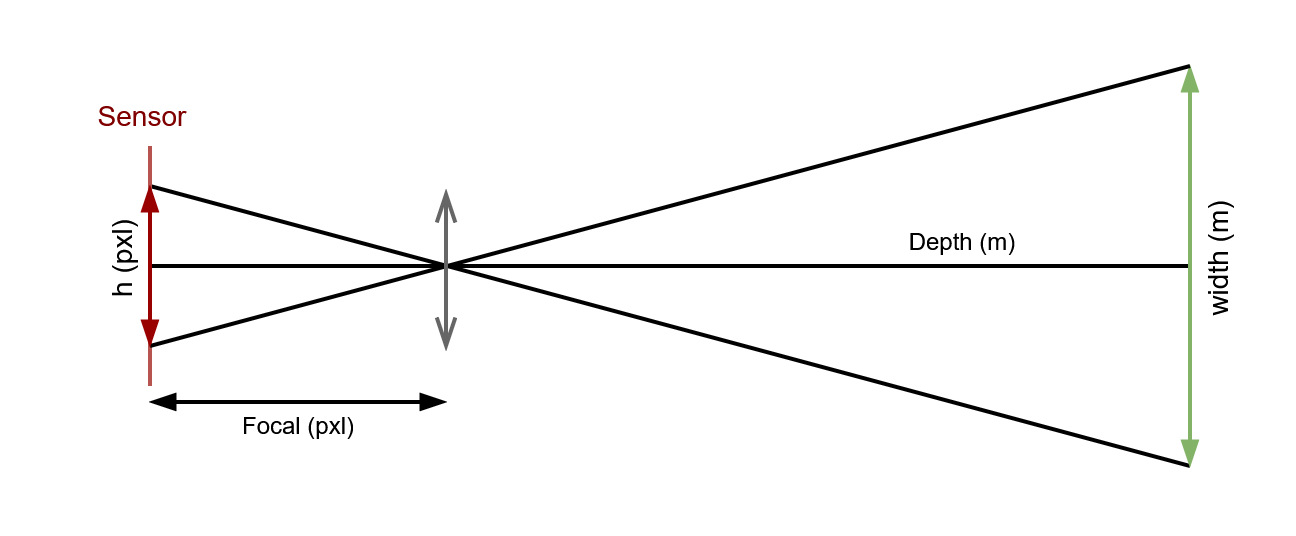
\includegraphics[width=0.45\textwidth]{images/app_photo_model.drawio.png}
    \caption{Hyopthèse de modélisation (simplifiée) de l'optique d'un appareil photo.}
    \label{fig:model-camera}
\end{figure}

\begin{equation} \label{eq:camera-relation}
    \frac{\text{width (pxl)}}{\text{focale (pxl)}} = \frac{\text{width (m)}}{\text{depth (m)}}
\end{equation}


et comme notre focale d'appareil est une constante, alors le produit $ \text{width} \times \text{depth} $  est proportionnel à la taille de la tête et doit donc être également répartie et ne pas dépendre de la prodonfeur, hors ce n'est pas ce que l'on observe, on voit en général nettement une correlation, comme sur notre exemple Figure \ref{fig:depth-correction} (gauche). 

\begin{figure}[h!]
    \centering
    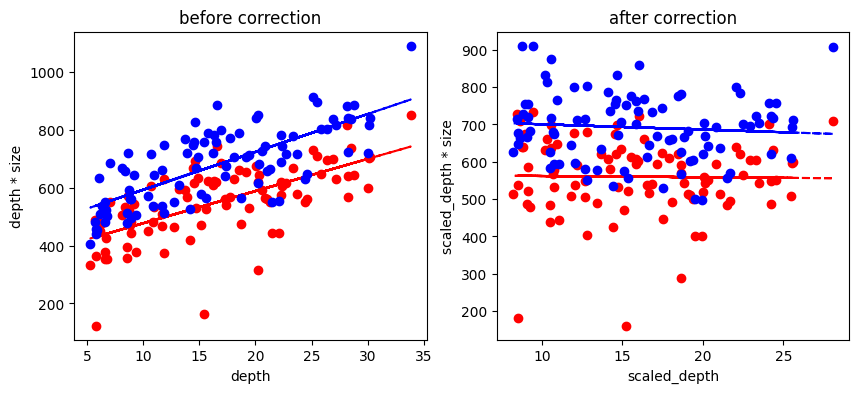
\includegraphics[width=0.45\textwidth]{images/depth_correction.png}
    \caption{(à gauche) avant la correction, on voit la corrélation. (à droite) la correction annule la correlation. }
    \label{fig:depth-correction}
\end{figure}

On effectue donc une régression linéaire pour déterminer une correctione linéaire à la carte de profondeur qui permet d'annuler la correlation entre le produit expliqué et la taille des têtes, comme on le vois figure \ref{fig:depth-correction} (droite).

On corrige ainsi la carte des profondeurs pour notre image (voir l'exemple Figure \ref{fig:depth-correction-example}).Sur notre exemple, on voit que l'échelle des profondeurs a été réduit, et que la distance maximum est passé à 50m ce qui est peut cohérent. Cependant comme on s'est concentré uniquement sur la région où sont disposé les têtes pour la correction, sur cette région la correction est plutôt cohérente (testé sur beaucoup d'images)

\begin{figure}
    \centering
    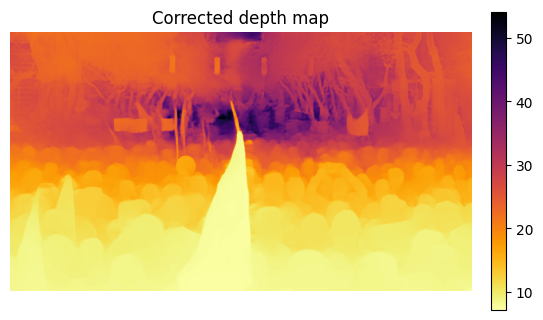
\includegraphics[width=0.45\textwidth]{images/result_depth_map_correction.png}
    \caption{Correction de la carte de profondeur sur notre exemple.}
    \label{fig:depth-correction-example}
\end{figure}

